\section{Experiments}
\subsection{Estimated Frequencies}
Roughly, estimated frequencies follow sigmoid growth. The exact growth is given by applying the transition function $t$ times.
\href{http://www.wolframalpha.com/input/?i=dx%2Fdt+%3D+s%2F2+%28x%281-x%29%29+%281%2F%281%2Bsx%29%29}{Writhing the ODE and Solving it gives}%
\beqn
  \frac{d\nu_t(s)}{dt} &=\frac{s}{2}\nu_t(s)(1-\nu_t(s))\frac{1}{1+s\nu_t(s)} \\
  \frac{st}{2}-c&=\log\left(\frac{\nu_t}{(1-\nu_t)^{1+s}}\right)   \label{eq:eactODE}
\eeqn
However we can not invert \ref{eq:exactODE} in closed form to get $\nu_t$ in terms of other quantities. In other words, the blue curve in the Figure \ref{fig:sigmoid} left, does not have a closed form inverse. But we can compute exact value of $\nu_t$ (and gradients of objective function w.r.t. $s$ ) in $\Oc(T)$. So no need to approximate even though the error is not significant Figure \ref{fig:sigmoid} Right.

\begin{figure}[H]
  \centering
    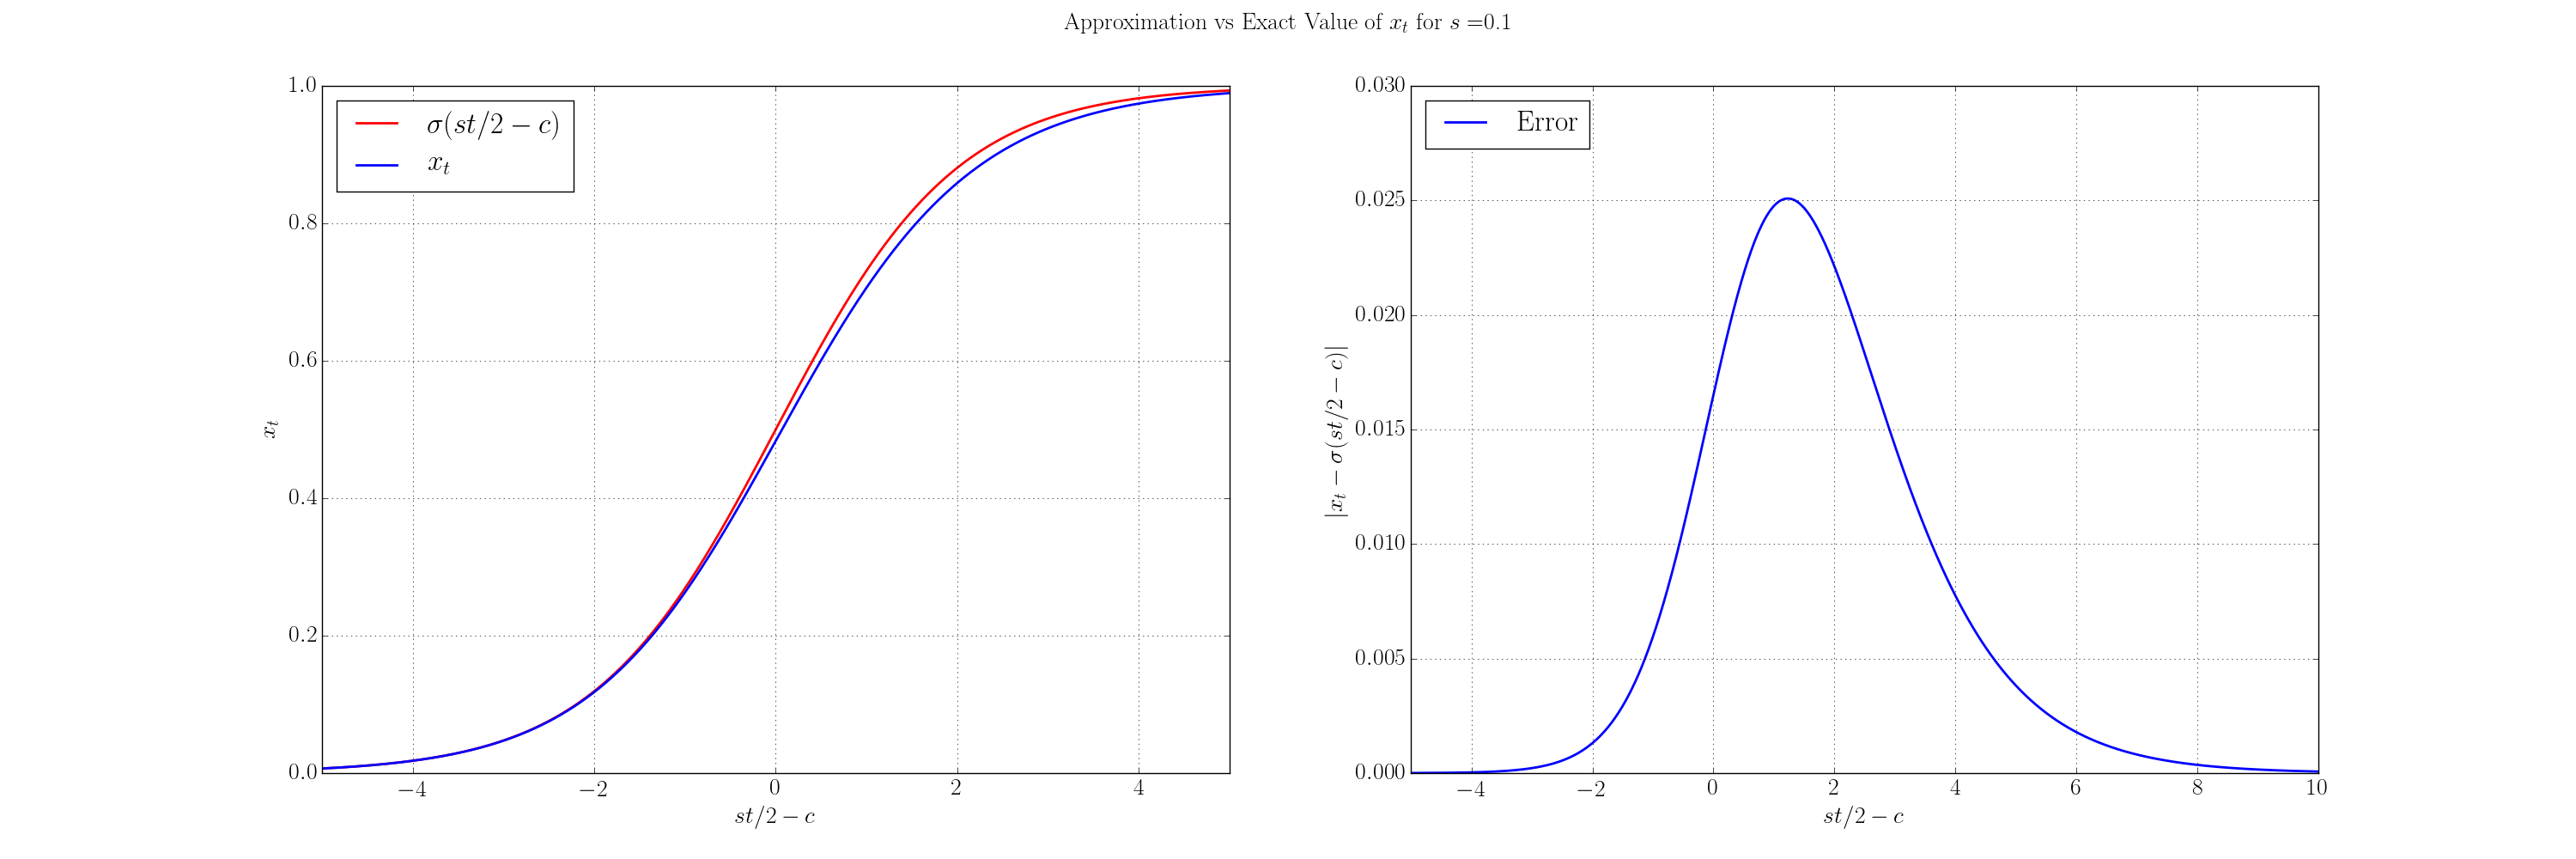
\includegraphics[width=\textwidth]{apprx}
  \caption{Rank}
  \label{fig:sigmoid}
\end{figure}

also $c \approx  \log(F)$ when minor allele is used for selection, i.e., $\nu_0=1/F$

\subsection{Understanding the difficulty of estimating $s$}
\subsubsection{Information Theory}
Signal to Noise Ration(SNR) is high when $s \rightarrow 0$ can be alleviated eliminating noise of genetic drift, i.e.  more replicates. 

\subsubsection{Functional Analysis}
The slope of sigmoid become close to zero as $s \rightarrow 0$, and can be alleviated by right choice of sampling in time.


\subsection{Data}
\subsubsection{Simulations}
For each experiment a diploid population is created and evolved as follows. 
\paragraph{I. Creating initial founder lines}
First using msms prgram, we created a population for $F$ founding haplotypes with parameters \texttt{\$./msms <F> 1 -t <4μLNe> -r <4Ne(L − 1)r> <L>} where $F=200$ is number of founder lines, 
$L=10^5$, $\theta=4\mu LNe=17$ and $\rho=4Ne(L-1)r=4$.  (assuming $Ne=1000$, $r=10^{-8}$ and $\mu=4.25\times 10^{-8}$).  
\paragraph{II. Creating initial diploid population} 
To mimic the real E\&R experiment for diploid organisms, first initial haplotypes cloned to create $F$ diploid homozygotes. Then each diploid is cloned $N/F$ times to yield $N$ diploid homozygote organisms.
\paragraph{III. Forward Simulation}
Given initial diploid population, position of the site under selection, selection strength $s$, number of replicates $R=3$, recombination rate $r=10^{-8}$ and sampling times $\Tc=\{10,20,30,40,50\}$ simuPop is used to perform forward simulation and compute allele frequencies for all of the $R$.

\subsubsection{Real}

\subsection{Likelihood Ratio Test}
Using the MLE (and other) estimates of $s$ it is desirable to perform a secondary task such as \emph{testing for selection} or \emph{locating the site under selection}. Likelihood ratio test (LRT) statistics for time series \cite{feder2014} have shown to be predictors for differentiating neutral and natural selection evolution cases. For a single locus model, the likelihood ratio test statistics $\Lambda(s*)$ is defined
\beq \label{eq:lrt}
\Lambda(s^*) = \log \left(\frac{\Lc(\bfX|s=s*)}{\Lc(\bfX|s=0)}\right)
\eeq
where $s^*$ is the optimal solution for the maximum-likelihood procedure. For the Gaussian process and Gaussian model the likelihood $\Lc_{GP}$ and $\Lc_G$ are well defined and \eqref{eq:lrt} can be easily evaluated. The likelihood of the Naive method for estimating based on $x_t$ is 
\beq
\Lc_N(s|x_t,x_0)=x_t-\sigma(st/2 -c)
\eeq

In addition to LRT, the value of $s^*$ itself can be regarded as a signal for detecting selection. In other words, modifying the LRT to
\beq
\Theta=s^*\Lambda(s^*)
\eeq
will take into account of two different objectives, 1)model discrepancy from neutral model 2)strength of selection under non-neutral model. In the  results we show that the modified-LRT makes more accurate predictions.

\subsection{Results}
In this part we compare the computational and predictive performance of the proposed method in detecting selection, locating selection in the genome, and estimating strength of selection with Gaussian process and the outlined naive method.

\subsubsection{Detecting Selection}
Detecting selection in the whole genome is a non-trivial task in real world and can be regarded as a application for the proposed algorithm. To provide a fair and unbiased comparison, we computed the test statistic for 1000 simulations and computed Receiver Operative Characteristic curve and Area Under Curve (AUC) for each method.



\begin{figure}[H]
  \centering
  \begin{tabular}{cc}
      \includegraphics[width=0.5\textwidth]{{roc0.01A0.01}.png} &    \includegraphics[width=0.5\textwidth]{{roc0.02A0.01}.png}\\
          \includegraphics[width=0.5\textwidth]{{roc0.05A0.01}.png}
&    \includegraphics[width=0.5\textwidth]{{roc0.1A0.1}.png}  
  \end{tabular}

  \caption{ROC}
  \label{fig:Fig3a}
\end{figure}

\begin{table}
\centering
\begin{tabular}{ l |c c c c }
$s$& 0.01 &0.02 & 0.05 & 0.1 \\
\hline
  Gaussian Model & 2 & 3& 2 & 3 \\
Gaussian Process & 5 & 6 & 2 & 3\\
  Naive & 8 & 9 & 2 & 3\\
\end{tabular}
\caption{AUC of all method evaluated for 1000 simulations and different values of $s$.}
\end{table}


\subsubsection{Finding Site Under Selection}
\paragraph{Distance}
\begin{figure}[H]
  \centering
    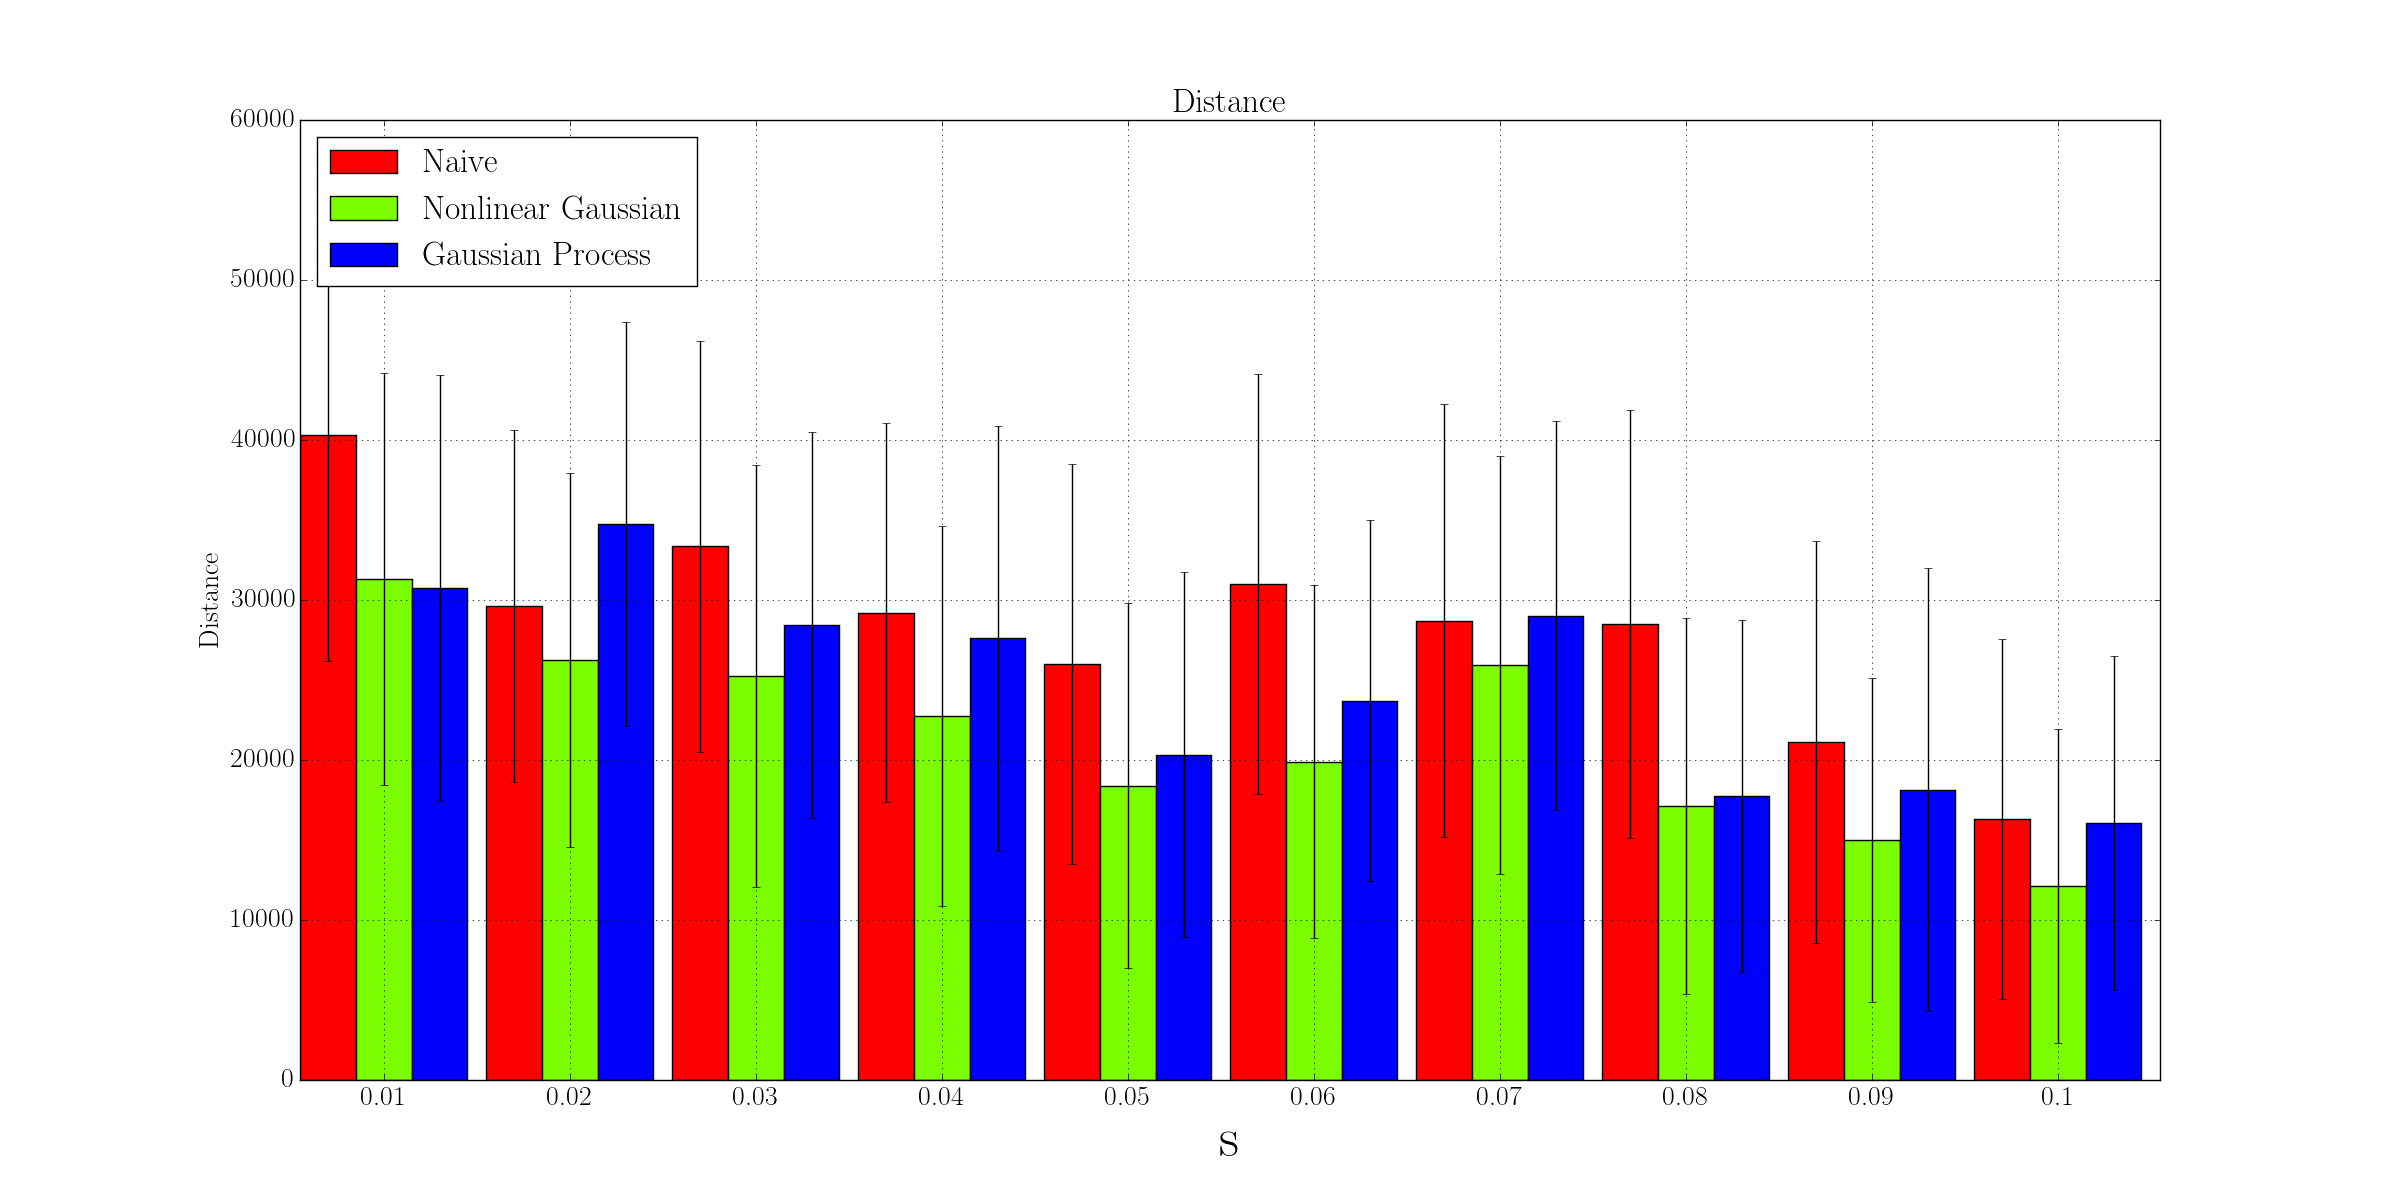
\includegraphics[width=\textwidth]{dist}
  \caption{Average distance to predicted site to the true site that is under selection.}
  \label{fig:Fig1}
\end{figure}

\paragraph{Rank}
\begin{figure}[H]
  \centering
    \begin{tabular}{c}
        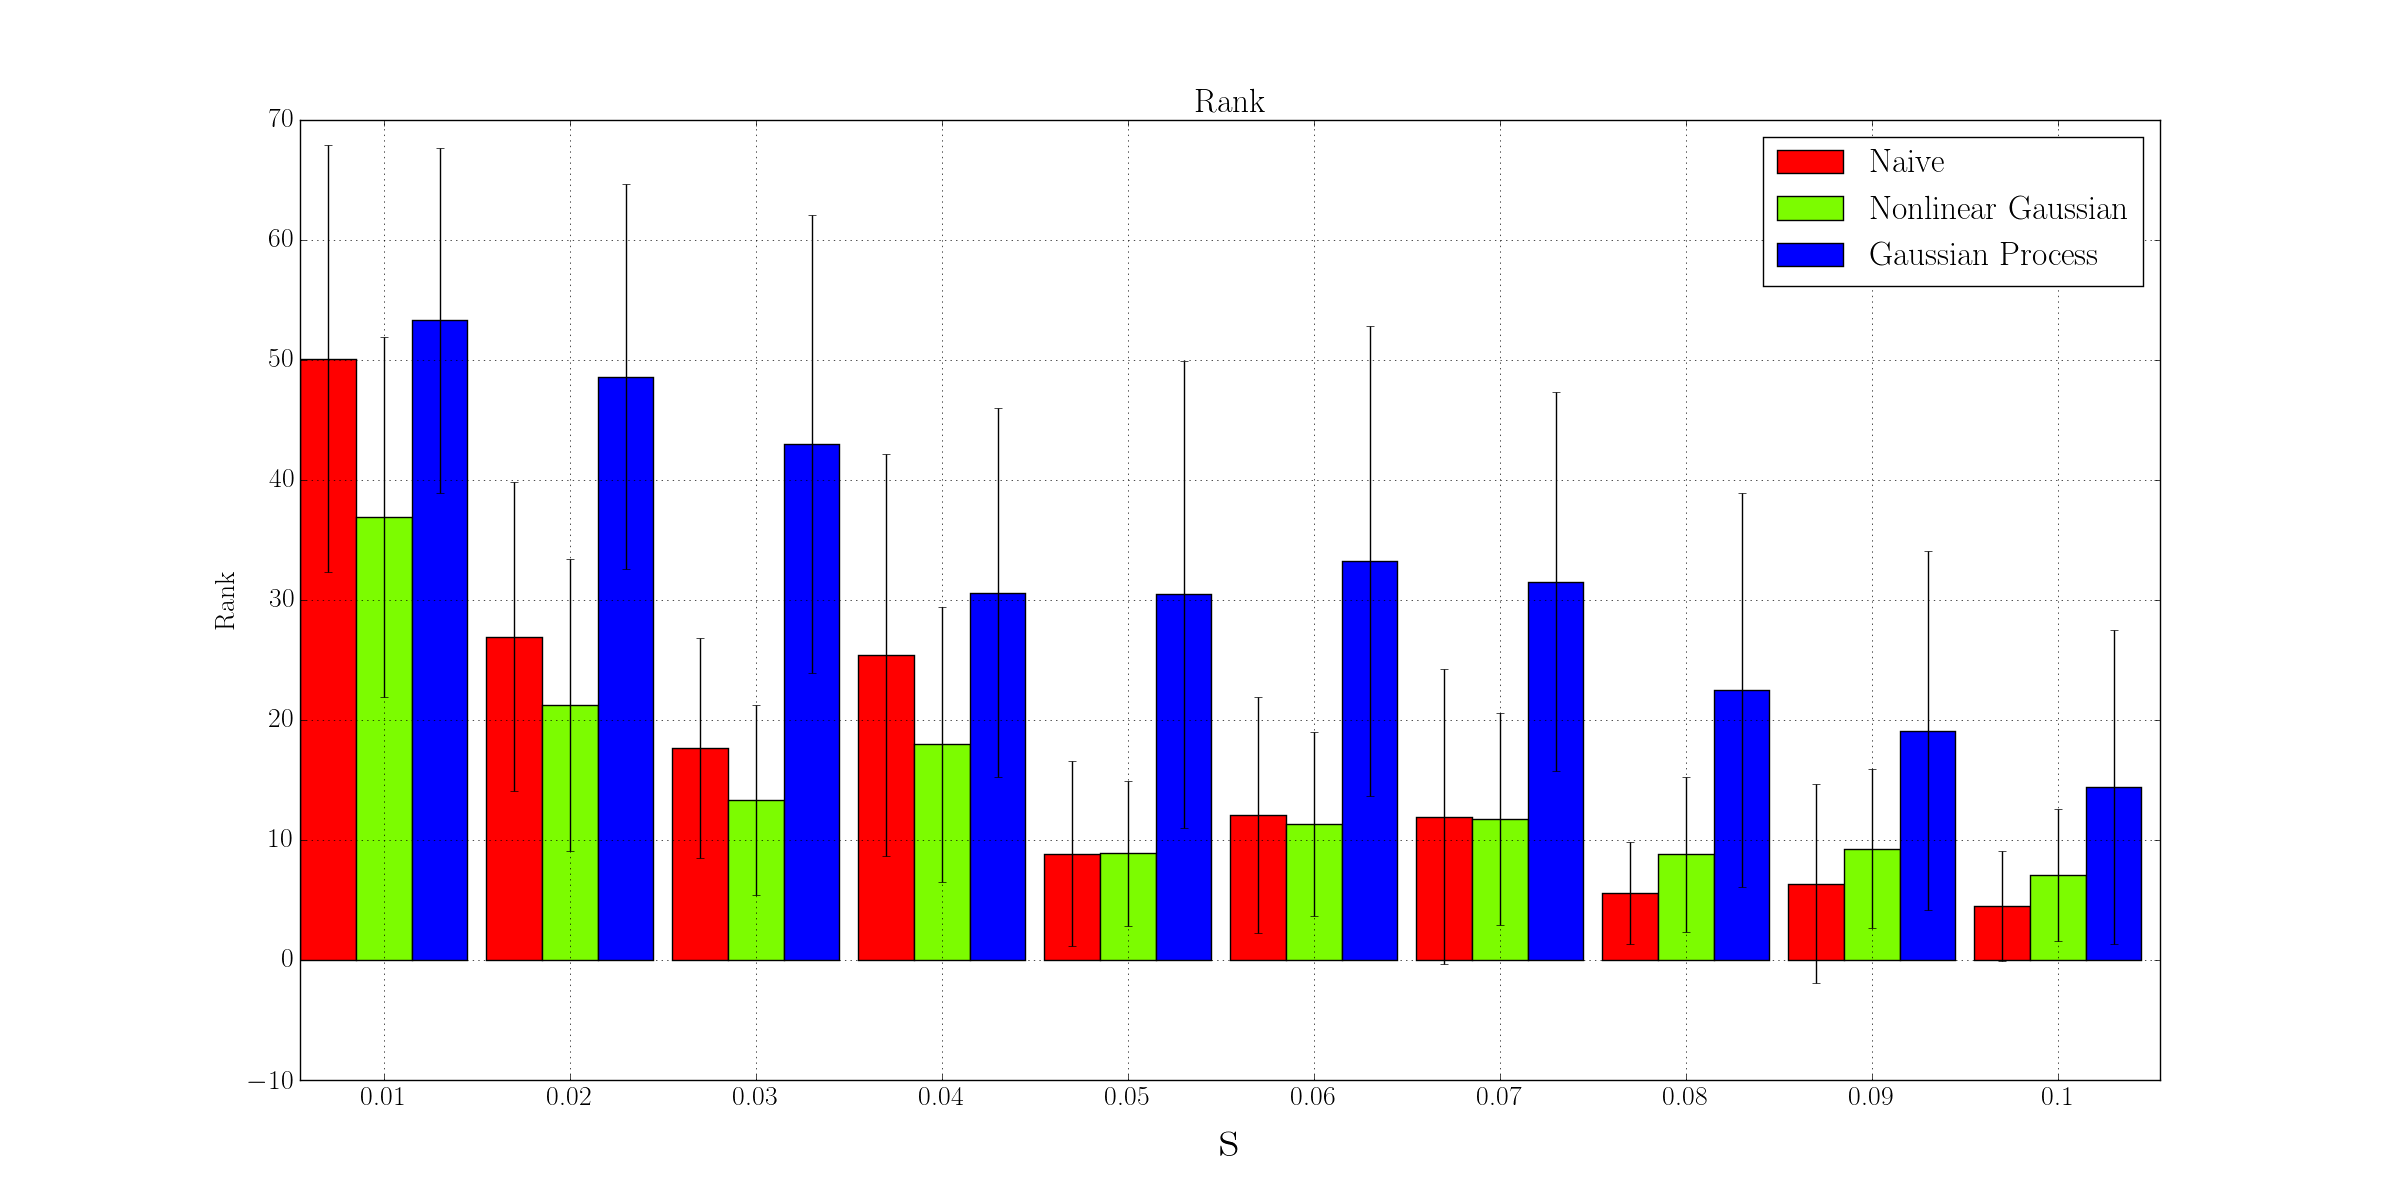
\includegraphics[width=0.8\textwidth]{rank}\\
  		    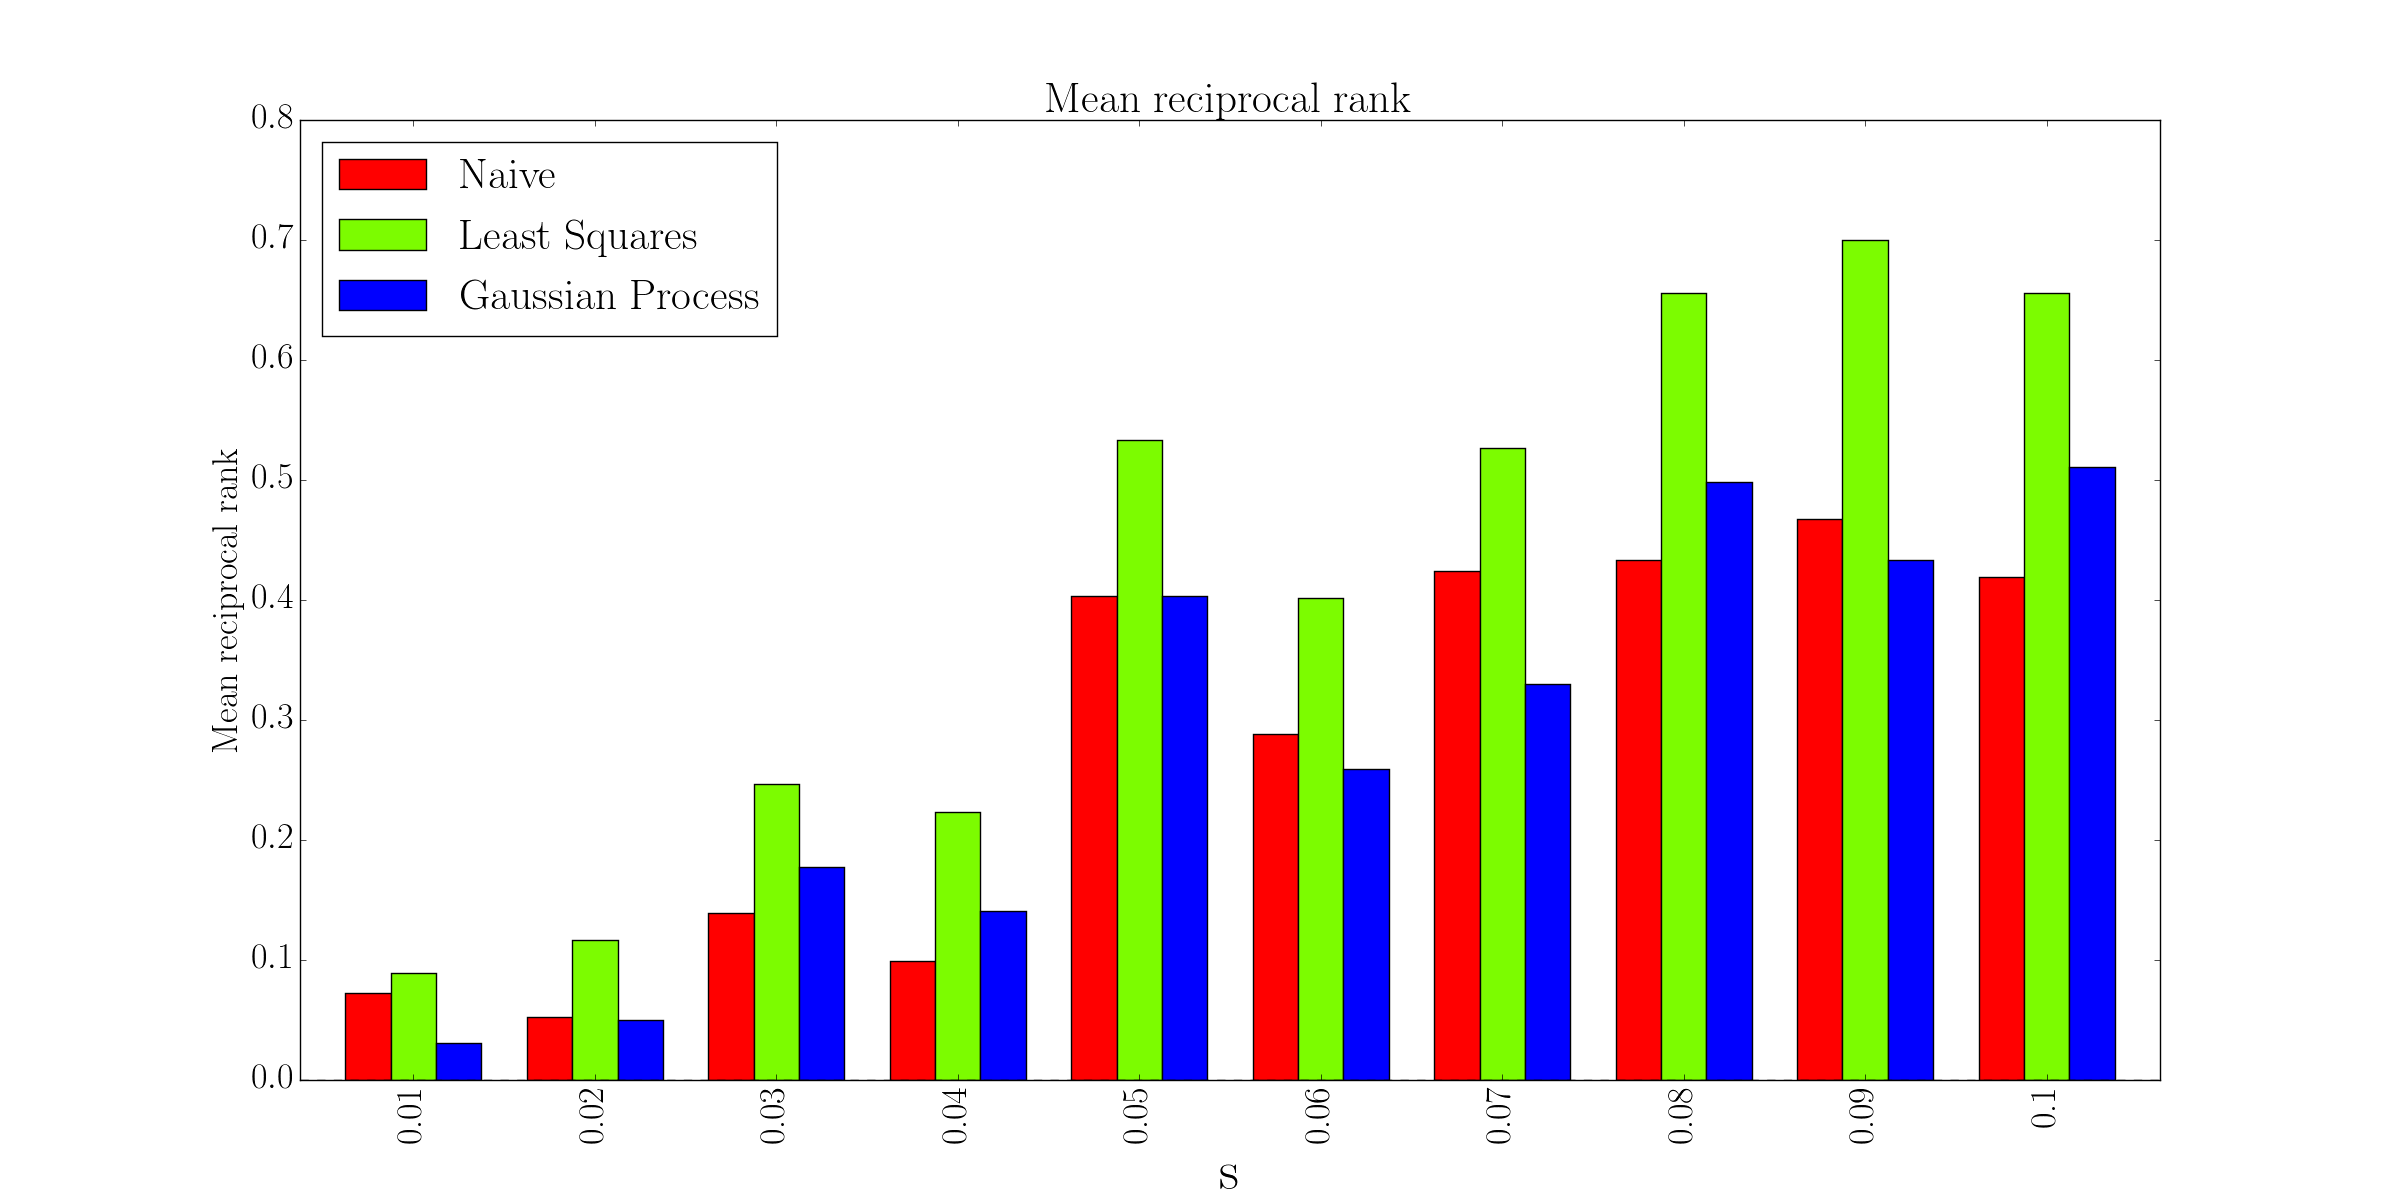
\includegraphics[width=0.8\textwidth]{mrr}\\
  		        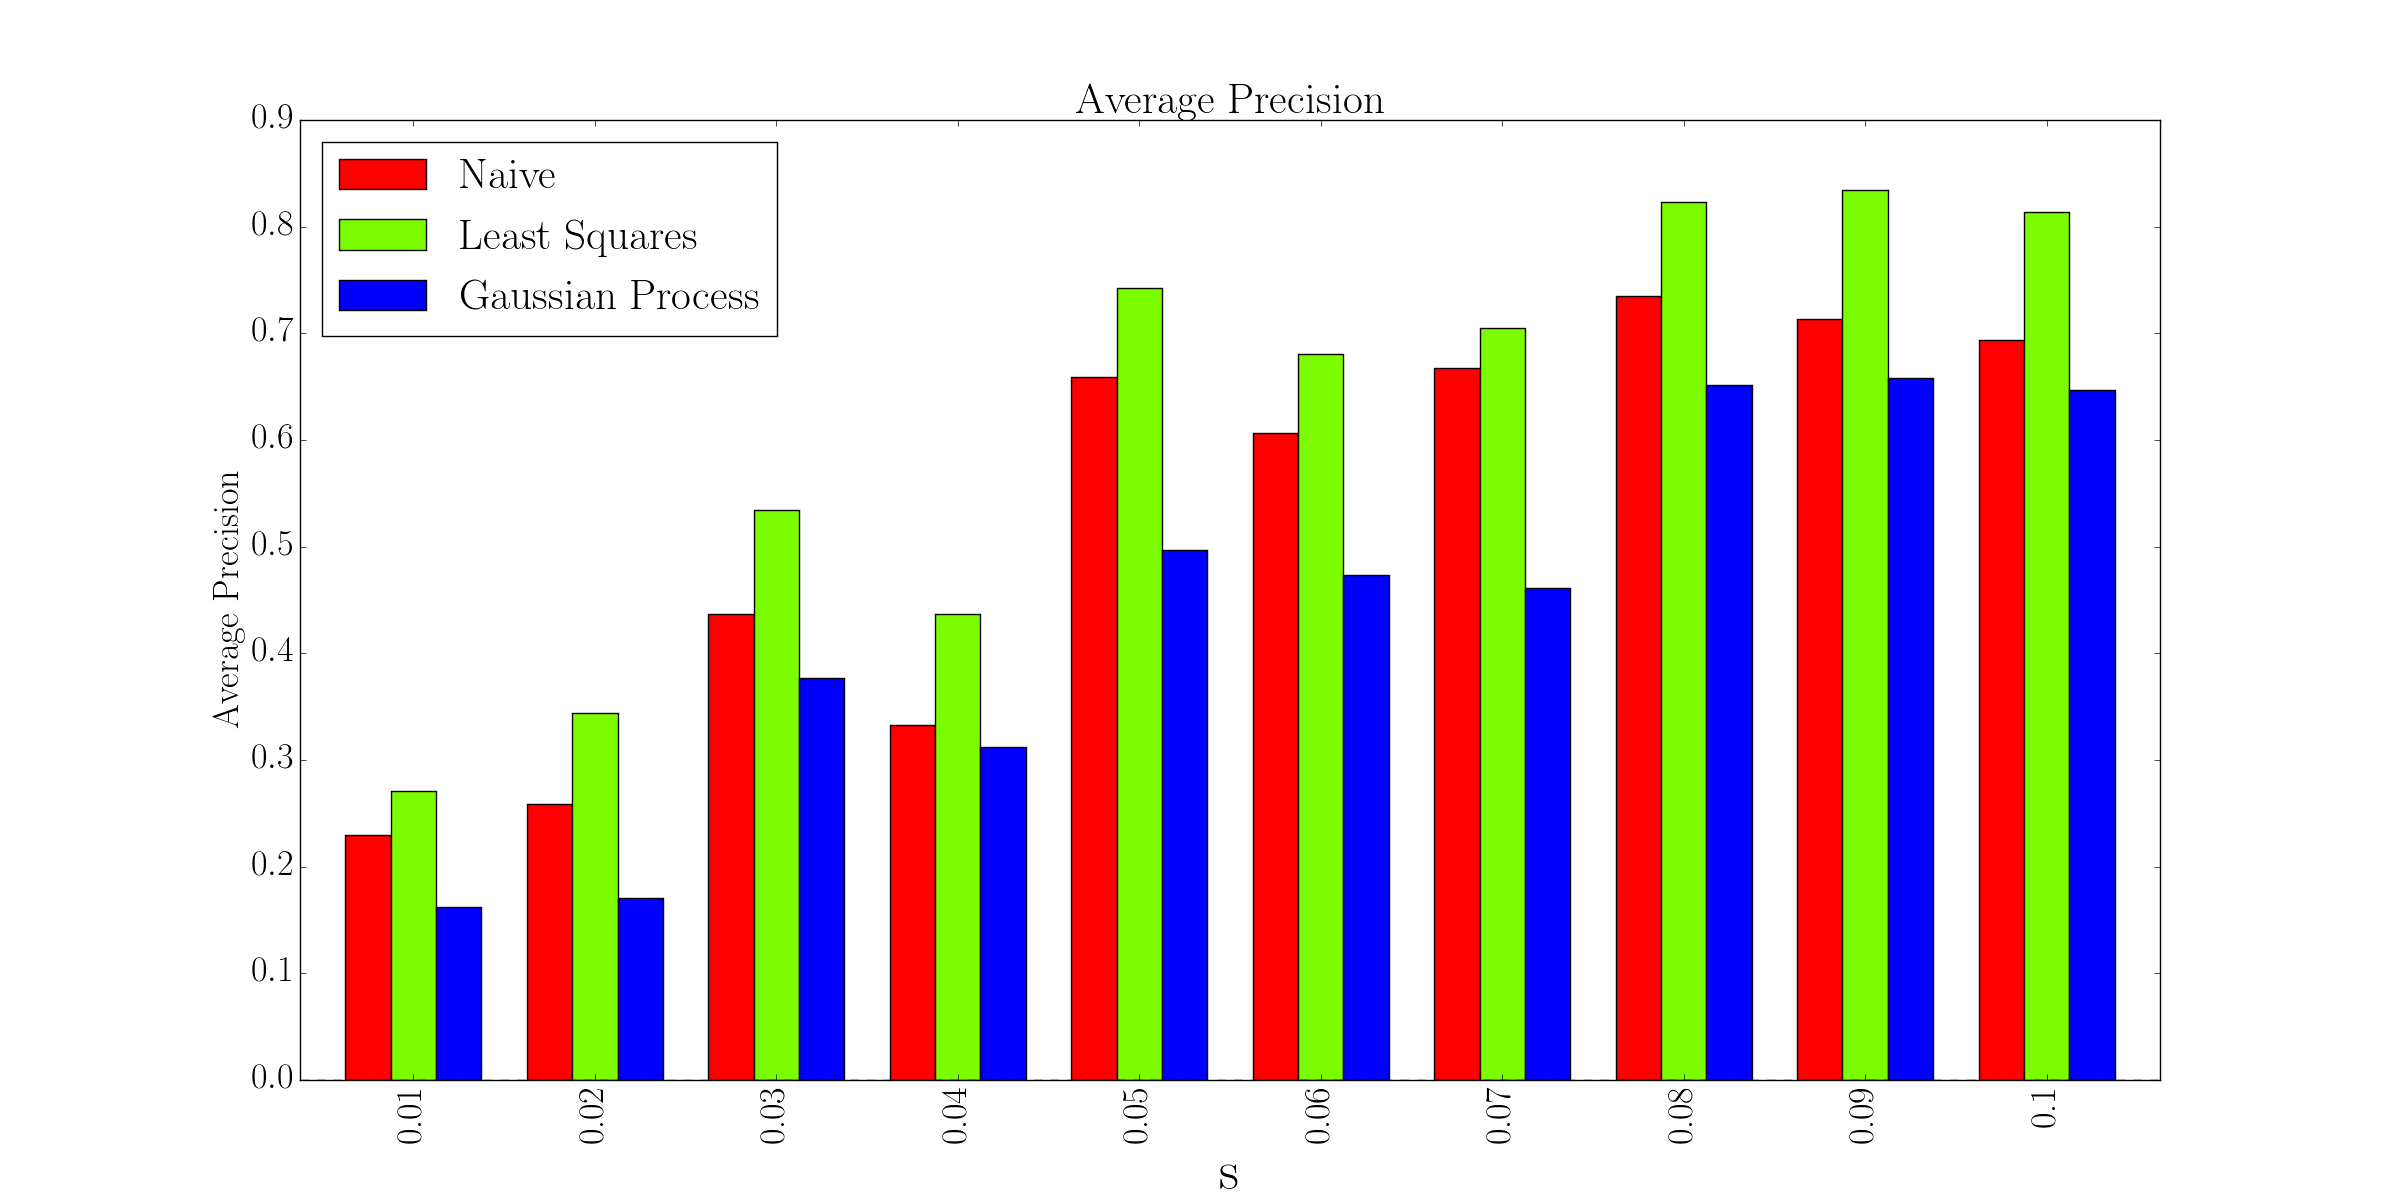
\includegraphics[width=0.8\textwidth]{ap}
  \end{tabular}
  \caption{Rank (Top), Mean Reciprocal Rank (Middle) Mean Average Precision (Bottom)}
  \label{fig:rank}
\end{figure}



\subsubsection{Estimating Strength of Selection}
\begin{figure}[H]
  \centering
    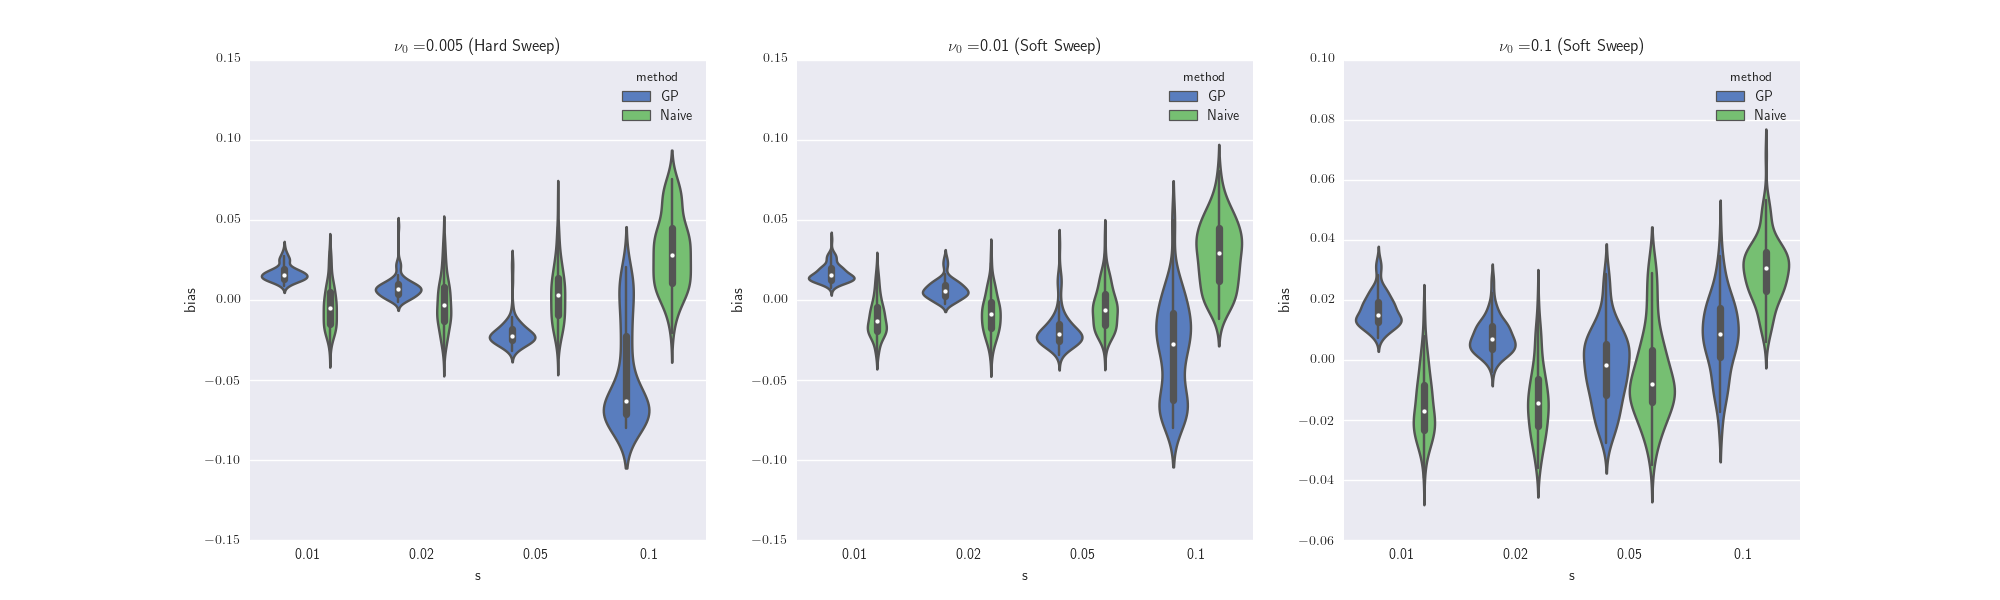
\includegraphics[width=\textwidth]{bias}
  \caption{Bias}
  \label{fig:Fig4}
\end{figure}

\subsection{Computational Performance}